\documentclass[12pt,a4paper]{article}
\usepackage[romanian]{babel}
\usepackage[utf8]{inputenc}
\usepackage[T1]{fontenc}
\usepackage{geometry}
\usepackage{graphicx}
\usepackage{hyperref}
\usepackage{float}
\usepackage{amsmath}
\usepackage{listings}

\geometry{margin=2.5cm}

\title{Lucrarea de laborator nr. 3\\
Sistem de monitorizare a duratei apăsărilor unui buton}
\author{Nume Prenume\\Grupa}
\date{\today}

\begin{document}
\begin{titlepage}
\begin{center}
\vspace*{1cm}
{\Large Technical University of Moldova}\\[0.5cm]
{\Large Faculty of Computers, Informatics and Microelectronics}\\[2cm]
{\Huge\bfseries Laboratory Work No. 2.2}\\[1cm]
{\Large\bfseries Embedded Systems:\\
Button Duration Monitor with Visual Signaling\\
and Periodic Reporting}\\[3.5cm]
\begin{flushright}
\begin{tabular}{ll}
\textbf{Elaborated:} & \\
std. gr. FAF-231 & Burduja Adrian \\[1cm]
\textbf{Verified:} & \\
asist. univ. & Alexei Martîniuc \\ & \\
\end{tabular}
\end{flushright}
\vfill
{\Large Chișinău -- 2026}
\end{center}
\end{titlepage}
\newpage

%-------------------------------------------------
\section{Task Analysis and Technological Context}

\subsection{Domain Analysis and Technological Context}
Multitasking embedded systems are widely used in monitoring applications,
human--machine interfaces, and real-time control. Monitoring the duration of an input action
(button press) is relevant in industrial systems, consumer electronics, and educational systems,
where the same physical interface may have different meanings depending on the interaction duration.

This work addresses this problem by implementing a multitasking system that clearly separates
data acquisition, statistical processing, and user reporting by leveraging the interface of the freeRTOS.

\subsection{External Resources and Bibliographic References}
The following types of resources were used:
\begin{itemize}
    \item documentation of the used microcontroller;
    \item documentation of the real-time operating system (RTOS);
    \item official examples regarding task management and timing;
    \item educational materials provided within the course.
    	\item Chat gpt for writting the structure of the report and some of the text
	\item Deepseek for helping with code
\end{itemize}


\subsection{Analysis of Components and Used Resources}
The system uses:
\begin{itemize}
    \item a microcontroller with multitasking support;
    \item a digital input push button;
    \item three LEDs (green, red, yellow);
    \item STDIO interface for reporting;
    \item software resources: tasks, logically protected global variables, and timers.
\end{itemize}

%-------------------------------------------------
\section{Definition of Technical Requirements and Test Scenarios}

\subsection{Application Objectives}
The main objective is the design and implementation of a multitasking application that:
\begin{itemize}
    \item detects button presses;
    \item measures their duration;
    \item visually signals the press type;
    \item collects statistics;
    \item periodically reports results.
\end{itemize}


\subsection{Functional and Non-Functional Requirements}

\textbf{Functional requirements:}
\begin{itemize}
    \item detection of press/release transitions;
    \item duration measurement in milliseconds;
    \item classification of presses into short and long;
    \item visual signaling using LEDs;
    \item periodic reporting via STDIO;
    \item statistics reset after reporting.
\end{itemize}

\textbf{Non-functional requirements:}
\begin{itemize}
    \item clear separation of responsibilities across tasks;
    \item temporal determinism;
    \item code readability and modularity;
    \item low resource consumption.
\end{itemize}

\subsection{Test Scenarios and Validation Criteria}
\begin{itemize}
    \item short press ($<500\,ms$) – green LED active;
    \item long press ($\geq500\,ms$) – red LED active;
    \item verification of the number of yellow LED blinks;
    \item correct reporting every 10 seconds;
    \item correct reset of statistics after reporting.
\end{itemize}

%-------------------------------------------------
\section{Architectural Design and Behavioral Modeling}

\subsection{System Components}
\begin{itemize}
    \item Detection Task – monitors the button and measures duration;
    \item Statistics Task – updates counters and yellow LED signaling;
    \item Reporting Task – sends data via STDIO;
    \item Hardware I/O – button and LEDs;
    \item STDIO Interface.
\end{itemize}

\newpage
\subsection{Structural Diagram}
\begin{figure}[!ht]
    
\includegraphics[width=0.8\textwidth]{img/structure.png}
    \caption{Architectural sketch}
\end{figure}

\subsection{HW--SW Layered Architecture}
The application is organized into the following layers:
\begin{itemize}
    \item hardware layer (button, LEDs);
    \item HAL layer (GPIO drivers, timing);
    \item RTOS layer (tasks, scheduler);
    \item application layer (logic and statistics).
\end{itemize}

\newpage
\subsection{Behavioral Diagrams}
\begin{figure}[!ht]
    \includegraphics[width=0.8\textwidth]{img/sequence.png}
    \caption{Behavioral sketch}
\end{figure}

%-------------------------------------------------
\newpage
\section{Electrical Schematic Design and Simulation}

\subsection{Electrical Schematic}
\begin{figure}[!ht]
    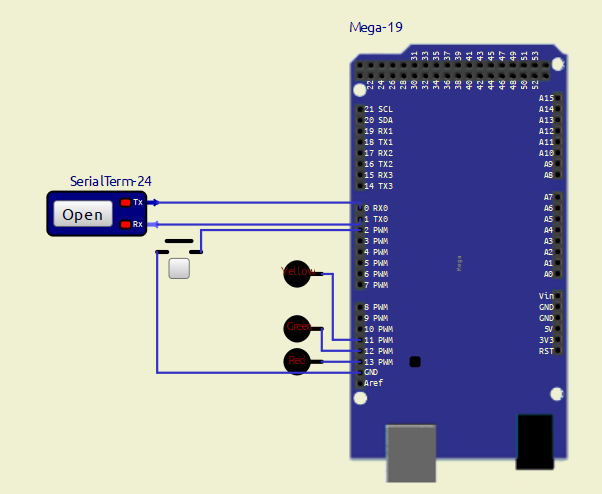
\includegraphics[width=0.8\textwidth]{img/sim.PNG}
    \caption{Behavioral sketch}
\end{figure}

\subsection{Connections and Component Sizing}
The button is connected to a digital input pin using a pull-up resistor, and the LEDs
are connected through appropriate current-limiting resistors.
\begin{figure}[!ht]
    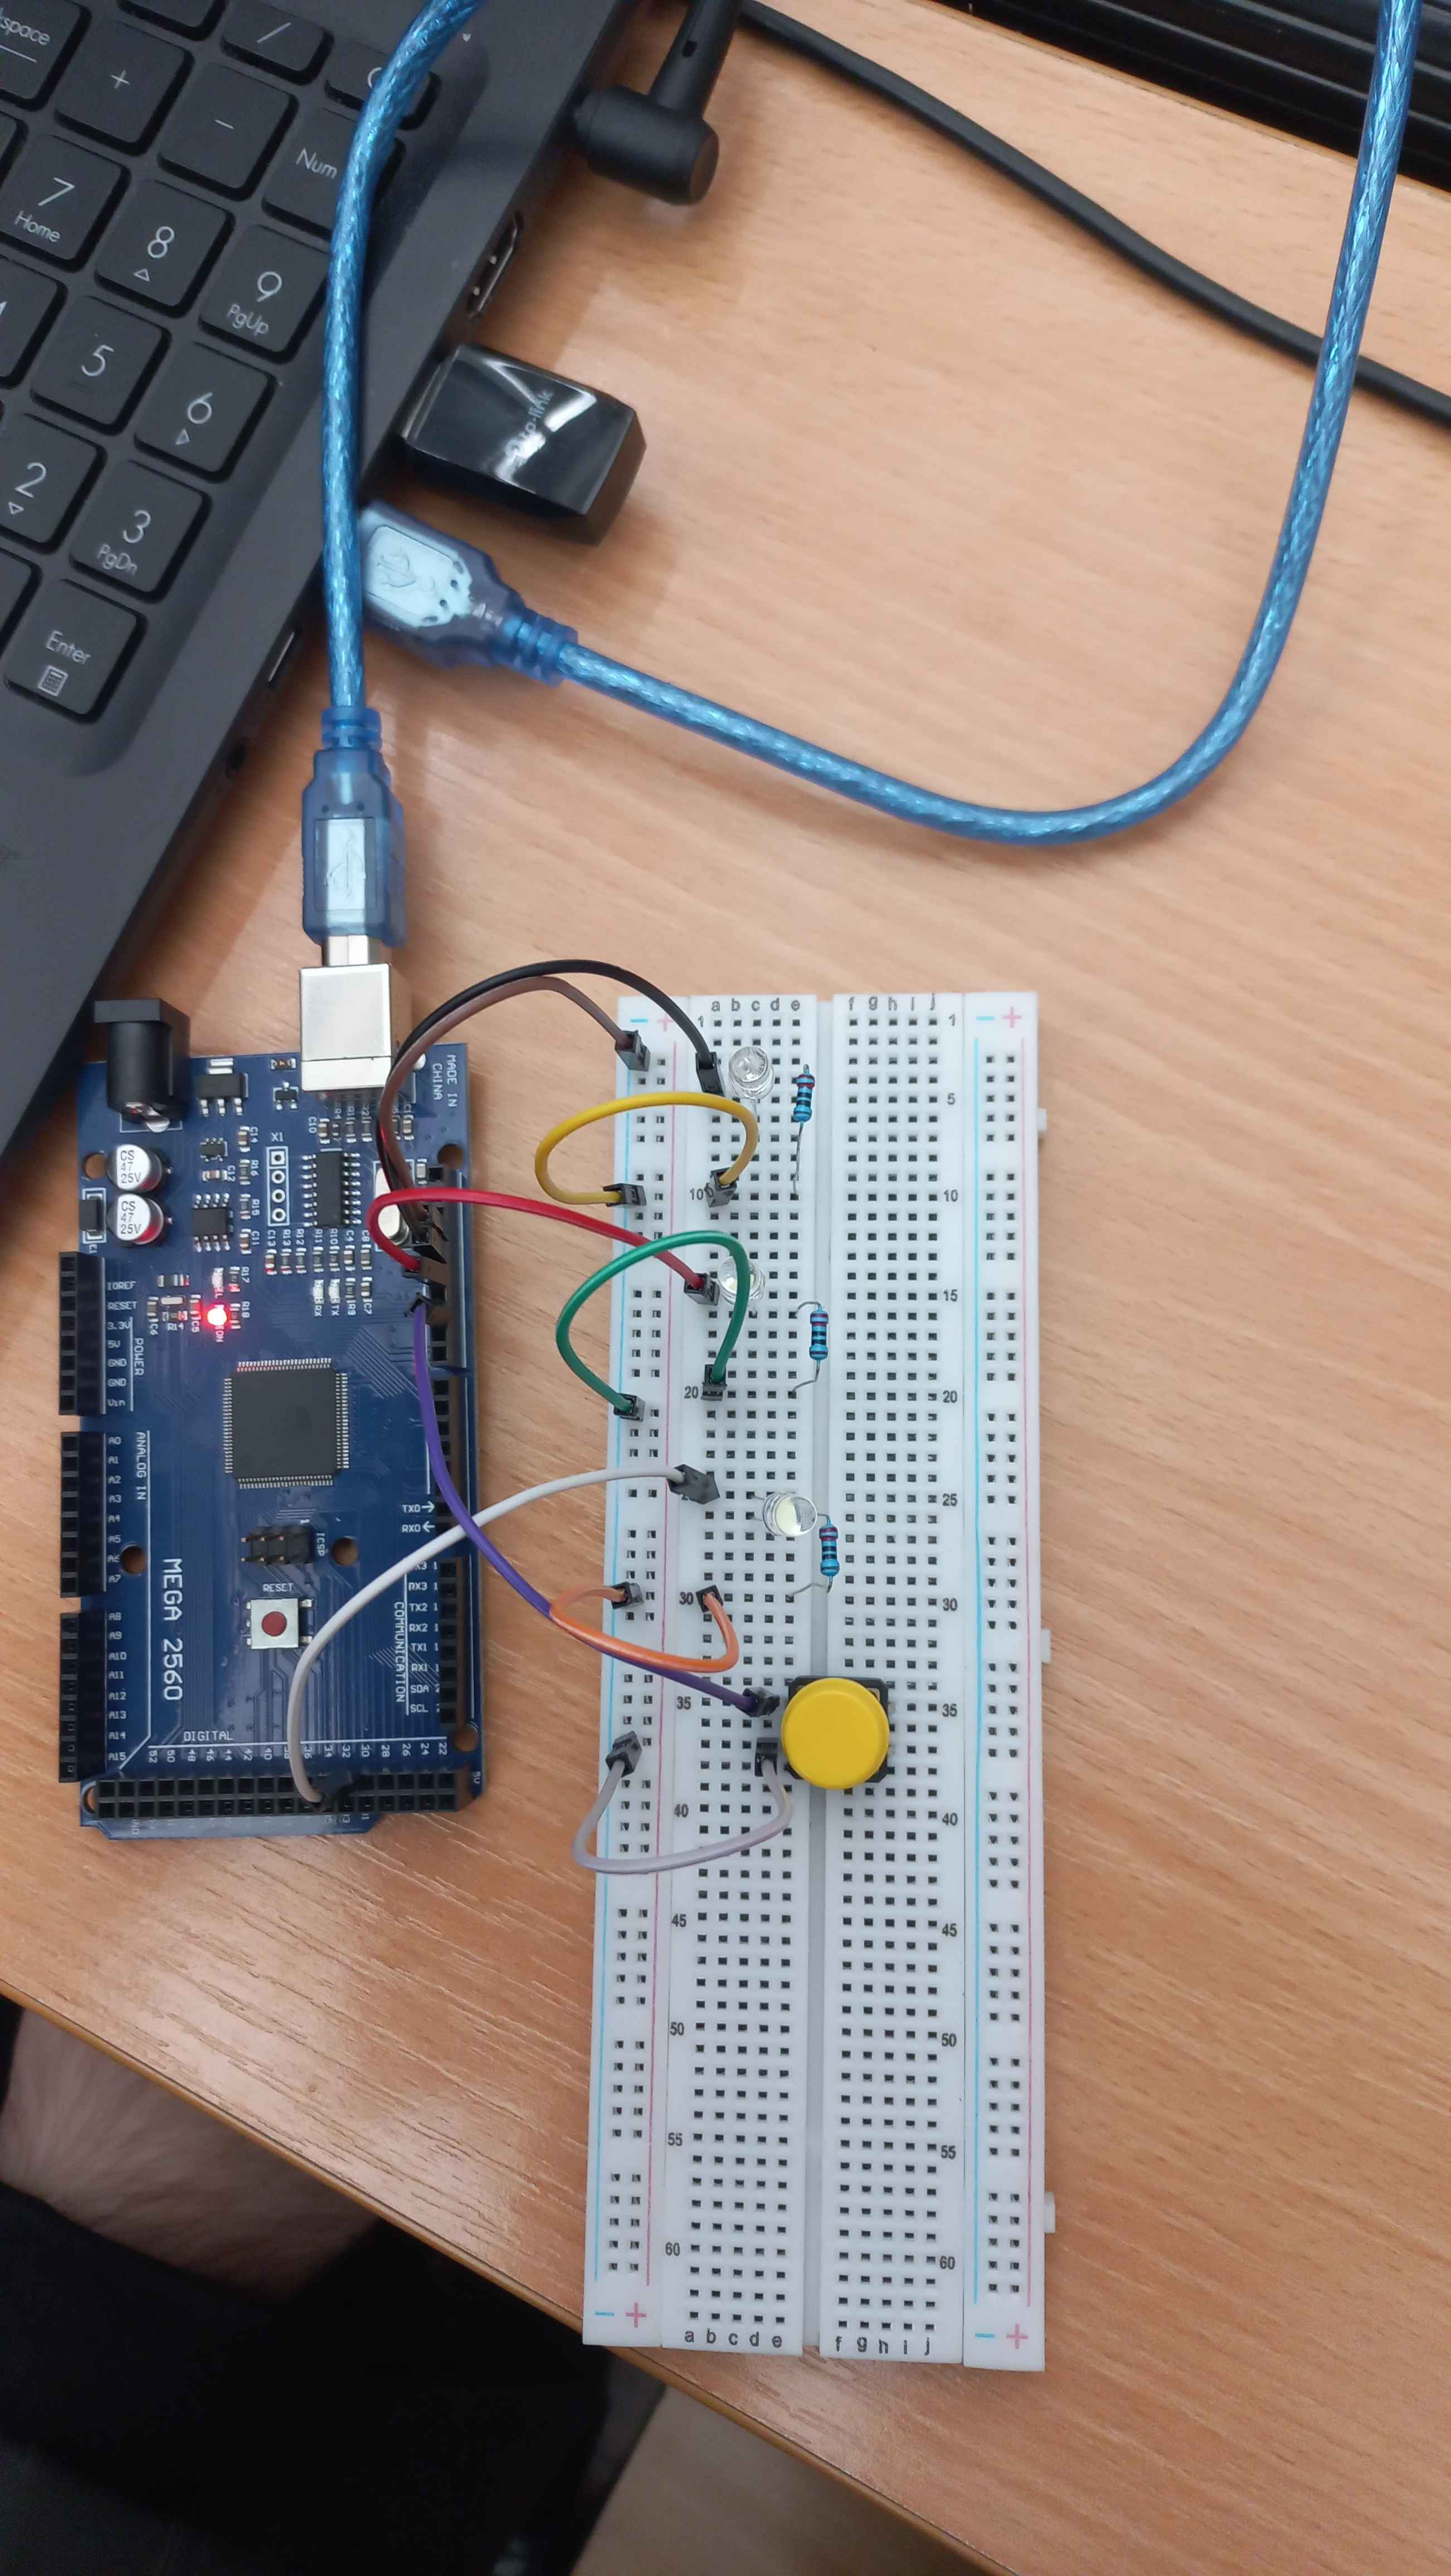
\includegraphics[width=0.8\textwidth]{img/board.jpg}
    \caption{Behavioral sketch}
\end{figure}

\subsection{Simulation}
The application was simulated in a virtual environment to validate logic and timing behavior. The simulator is called SimulIDE.

\subsection{Execution on Real Hardware}
Results of running the application(terminal output):
\begin{lstlisting}
Numarul de apasari: 2
Numarul de apasari scurte: 1
Numarul de apasari lungi:  1
Durata medie a apasarilor: 343
\end{lstlisting}

%-------------------------------------------------
\section{Modular Software Implementation}

\subsection{Project Structure}
\begin{lstlisting}
build\
rtos.ino
build.bat
button_driver.c
button_driver.h
leds_driver.c
leds_driver.h
main.c
stdio_layer.c
stdio_layer.h
task_procs.c
task_procs.h
\end{lstlisting}



\subsection{HW--SW Interface}
Dedicated functions are used for GPIO access and timing, separated from the application logic.

\subsection{Behavior Implementation}
Each task implements a clearly defined role, according to the initial design.

\subsection{Comments and Documentation}
The code is commented to highlight the logic and design decisions.

%-------------------------------------------------
\section{Simulation, Testing, and Validation}

\subsection{Testing}
Tests were performed according to the previously defined scenarios.

\subsection{Results and Observations}
The obtained results confirm the correct operation of the application.

\subsection{Optimizations}
Optimizations related to timing and task organization were identified.

%-------------------------------------------------
\section{Conclusions}

The developed application demonstrates the effective use of multitasking in an embedded system.
Separating functionality across tasks improves clarity, scalability, and system reliability.
The solution can be easily extended for more complex applications.

\newpage
\section{Annex}

\subsection{ button\_driver.c }
\begin{lstlisting}
#include "button_driver.h"
#include <Arduino.h>

#define BUTT_PIN 2

void init_button()  { pinMode(BUTT_PIN, INPUT_PULLUP); }
bool button_state() { return digitalRead(BUTT_PIN);    }
\end{lstlisting}

\subsection{button\_driver.h}
\begin{lstlisting}
#pragma once

#include <stdbool.h>
void init_button();

bool button_state();
\end{lstlisting}

\subsection{leds\_driver.c}
\begin{lstlisting}
#include "leds_driver.h"
#include <Arduino.h>

// Register controll
#define RED_LED_PIN 13
#define GREEN_LED_PIN 12
#define YL_LED_PIN 11

void init_leds(){
	pinMode(RED_LED_PIN,   OUTPUT);
	pinMode(GREEN_LED_PIN, OUTPUT);
	pinMode(YL_LED_PIN,    OUTPUT);

	yl_led_turn_off();
	red_led_turn_off();
	green_led_turn_off();
}

void red_led_turn_on()  { digitalWrite(RED_LED_PIN,HIGH); }
void red_led_turn_off() { digitalWrite(RED_LED_PIN, LOW); }

void green_led_turn_on()  { digitalWrite(GREEN_LED_PIN,HIGH); }
void green_led_turn_off() { digitalWrite(GREEN_LED_PIN, LOW); }

void yl_led_turn_on()  { digitalWrite(YL_LED_PIN,HIGH); }
void yl_led_turn_off() { digitalWrite(YL_LED_PIN, LOW); }

\end{lstlisting}

\subsection{leds\_driver.h}
\begin{lstlisting}
#pragma once

#include <stdbool.h>
void init_leds();
void init_button();

void red_led_turn_on();
void red_led_turn_off();
void green_led_turn_on();
void green_led_turn_off();
void yl_led_turn_on();
void yl_led_turn_off();

bool button_state();
\end{lstlisting}

\subsection{main.c}
\begin{lstlisting}
#include <Arduino.h>
#include "task_procs.h"


int main(void){
	init();
	init_tasks();

	for(;;){ }

	return 0;
}
\end{lstlisting}

\subsection{stdio\_layer.c}
\begin{lstlisting}
#include "stdio_layer.h"
#include <stdio.h>
#include <Arduino.h>
// Code generated by claude
// start

int uart_putchar(char c, FILE *stream) {
	if (c == '\n') { uart_putchar('\r', stream); }
	while(!(UCSR0A & (1 << UDRE0)));
	UDR0 = c;
	return 0;
}

int uart_getchar(FILE *stream) {
	while(!(UCSR0A & (1 << RXC0)));
	return UDR0;
}

FILE uart_str = FDEV_SETUP_STREAM(uart_putchar, uart_getchar, _FDEV_SETUP_RW);

void uart_init(unsigned long baud){
	unsigned int ubrr = F_CPU/16/baud - 1;
	UBRR0H = (ubrr >> 8);
	UBRR0L = ubrr;
	UCSR0B = (1 << TXEN0) | (1 << RXEN0);
	UCSR0C = (3 << UCSZ00);

	stdout = &uart_str;
	stdin = &uart_str;
}

// end

void init_stdout(){ uart_init(9600); }

// IO
#define BUFFER_SIZE 255
char _buffer[BUFFER_SIZE+1];
char* buffer(){return _buffer;}

int _bufflen = 0;
int bufflen(){return _bufflen;}

void read_input(){
	fgets(_buffer, BUFFER_SIZE, stdin);
	_bufflen = strlen(_buffer);
}

void print_input(){ printf("%s", _buffer); }
\end{lstlisting}

\subsection{stdio\_layer.h}
\begin{lstlisting}
#pragma once
#include <stdio.h>

// forward decl for Arduino.h function
int strncmp(const char *, const char *, unsigned int);

void uart_init(unsigned long baud);
int uart_putchar(char c, FILE *stream);
int uart_getchar(FILE *stream);

char* buffer();
int bufflen();

void init_stdout();

void read_input();
void print_input();
\end{lstlisting}

\subsection{task\_procs.c}
\begin{lstlisting}
#include <Arduino_FreeRTOS.h>
#include <queue.h>
#include <stdio.h>

#include "Arduino.h"

#include "task_procs.h"
#include "button_driver.h"
#include "leds_driver.h"
#include "stdio_layer.h"

typedef struct {
	unsigned long sum_shorts,sum_longs;
	int presses, n_shorts,n_longs;
}stats_t ;

QueueHandle_t duration_queue;
QueueHandle_t stats_queue;
void init_tasks(){
	init_button();
	init_leds();
	init_stdout();

	duration_queue = xQueueCreate(10,sizeof(unsigned long));
	stats_queue = xQueueCreate(10,sizeof(stats_t));

	xTaskCreate(task1_proc, "Task1", 128, NULL, 2, NULL);
	xTaskCreate(task2_proc, "Task2", 128, NULL, 1, NULL);
	xTaskCreate(task3_proc, "Task3", 128, NULL, 1, NULL);
	vTaskStartScheduler();
}

// manage press intervals
void task1_proc(void* pvParameters){
	(void)pvParameters;

	for (;;){
		// while button has not been pressed, wait
		while (button_state() == HIGH ) { vTaskDelay(1); }
		
		unsigned long start = millis();

		// while the button is still held, wait
		while (button_state() == LOW) { vTaskDelay(1); }

		unsigned long finish = millis();
		unsigned long duration = finish - start;

		// notify task2 that there is data to consume
		//		//xQueueSend copies the data internally
		xQueueSend(duration_queue, &duration, 0);

		if (duration < 500){
			// short hold
			green_led_turn_on();
			red_led_turn_off();
		} else {
			// long hold
			red_led_turn_on();
			green_led_turn_off();
		}
	}
}

#define LONG_PRESS 500
// manage press statistics
void task2_proc(void* pvParameters){
	(void)pvParameters;

	for (;;){
		unsigned long duration = 0;

		xQueueReceive(duration_queue, &duration,portMAX_DELAY);

		// process the input
		stats_t stats = {0}; 
		stats.presses +=1;
		int blink_n = 0;
		if (duration < LONG_PRESS) {
			stats.sum_shorts += duration;
			stats.n_shorts += 1;
			blink_n = 5;
		} else {
			stats.sum_longs += duration;
			stats.n_longs += 1;
			blink_n = 10;
		}

		xQueueSend(stats_queue, &stats, 0);

		// blink blink_n times
		for (/**/; blink_n>0; blink_n-=1) {
			yl_led_turn_on();
			vTaskDelay(pdMS_TO_TICKS(100));
			yl_led_turn_off();
			vTaskDelay(pdMS_TO_TICKS(100));
		}

	}
}


#define REPORT_INTERVAL 10

void task3_proc(void* pvParameters){
	(void)pvParameters;

	for(;;){
		vTaskDelay(pdMS_TO_TICKS(REPORT_INTERVAL*1000));
		stats_t total_stats = {0};
		BaseType_t recieved;

		// process all the items in the queue imediately
		do {
			stats_t stats = {0}; 
			recieved = xQueueReceive(stats_queue, &stats, 0);
			total_stats.presses += stats.presses;
			total_stats.n_longs += stats.n_longs;
			total_stats.n_shorts += stats.n_shorts;
			total_stats.sum_longs += stats.sum_longs;
			total_stats.sum_shorts += stats.sum_shorts;
		
		}while (recieved != pdFALSE);

		unsigned long averege_holds = total_stats.sum_longs + total_stats.sum_shorts;
		
		if (total_stats.presses > 0) {
			averege_holds = averege_holds / (total_stats.presses);
		}

		printf(
			"Numarul de apasari: %d\n"
			"Numarul de apasari scurte: %d\n"
			"Numarul de apasari lungi:  %d\n"
			"Durata medie a apasarilor: %lu\n",
			total_stats.presses,
			total_stats.n_shorts,
			total_stats.n_longs,
			averege_holds
		);

	}
}
\end{lstlisting}

\subsection{task\_procs.h}
\begin{lstlisting}
#pragma  once

void init_tasks();
\end{lstlisting}


\end{document}